\documentclass[11pt]{article}

\usepackage[utf8]{inputenc}
\usepackage[T1]{fontenc}
\usepackage[margin=1in]{geometry}
\usepackage{graphicx}
\usepackage{booktabs}
\usepackage{amsmath,amssymb}
\usepackage{array}
\usepackage[labelfont=bf,font=small]{caption}
\usepackage{xcolor}
\usepackage{enumitem}
\usepackage{float}
\usepackage[hidelinks]{hyperref}

\graphicspath{{figures/}}
\setlength{\parskip}{0.4em}
\setlength{\parindent}{0pt}
\newcommand{\sig}[1]{\texttt{#1}}

\title{\textbf{Can Large Language Models Extract Cross-Sectional Equity Signals\\
from SEC Annual-Report Narratives?}\\[0.4em]
\large A Validity-Driven Study Across Eleven Experimental Rounds}

\author{Allison}
\date{November 2026}

\begin{document}
\maketitle

\begin{abstract}
\noindent
This report asks whether a large language model (LLM) reading the narrative sections of
SEC 10-K filings can produce a signal that forecasts short-horizon relative equity returns.
The study is organised as eleven experimental rounds. Each round exists to close one
specific threat to the validity of the previous round's conclusion, rather than to try a
new idea; more than half of the rounds changed how the result was \emph{measured} rather
than what was measured. The final design pairs a deterministic year-over-year text diff
with an LLM that judges only whether a change is material, and evaluates the resulting
signal through a sector-neutral rank-weighted long--short portfolio against three
independent checks: a persistent neutralised random baseline, a Fama--French factor
regression with Newey--West standard errors, and a sixfold expansion of the sample.

Three findings survive. First, at full statistical power the LLM ``diff-surprise'' signal
on Item 1A Risk Factors is \emph{significantly negative} ($-0.83$ Sharpe; FF3+MOM alpha
$-8.9\%$/yr, $t=-2.54$), worse than all 500 random baselines, and it reverses a positive
result ($+0.57$ Sharpe, alpha $p=0.045$) obtained on a smaller sample. Second, the
failure is traceable to a structural negativity bias: the model used the full negative
half of its permitted score range and never the top of the positive half. Third, moving
the text source to the MD\&A section did not rescue the approach---a pre-registered
Lazy-Prices-style similarity hypothesis came out significantly \emph{opposite} in sign
($-0.72$ Sharpe, alpha $t=-2.95$), a result that is robust within sample but is most
plausibly survivorship bias in a current-membership universe.

The contribution is therefore not a profitable signal. It is a reusable validation
framework, a documented record of the measurement errors it caught---including a parser
defect affecting 42\% of inputs and a filing-coverage defect that silently thinned the
early cross-section to single digits---and a clean, well-powered negative answer to a
question the literature leaves open.
\end{abstract}

\tableofcontents
\newpage

%=======================================================================
\section{Introduction}

\subsection{Motivation}

Public companies are legally required to describe, in narrative form, what could go wrong
with their business (Item 1A, ``Risk Factors'') and how management reads its own results
(Item 7, ``Management's Discussion and Analysis'', or MD\&A). These sections are long,
unstructured, and written by lawyers. They are also, in principle, the most explicitly
forward-looking text a firm publishes on a fixed schedule.

Two literatures meet here. Accounting research has established that risk-factor
disclosure is firm-specific and informative, and that \emph{changes} in filing language
from one year to the next carry return-relevant information. Separately, the recent
LLM-in-finance literature has shown that language models can extract tradable sentiment
from text. The obvious intersection---use an LLM to read the year-over-year change in a
firm's risk narrative---has not, to our knowledge, been tested under proper
cross-sectional controls.

The intersection is attractive precisely because it is cheap to reach: the data is free
and public, the filing date gives an unambiguous point-in-time anchor, and the
year-over-year structure means the model can be asked a narrow, well-posed question
(``what is new, and does it matter?'') rather than an open-ended one.

\subsection{Research question}

\begin{quote}
\textbf{Can structured signals extracted by an LLM from SEC annual-report narratives
forecast short-horizon relative stock returns, and do they beat a transparent lexicon
baseline on identical data and identical portfolio construction?}
\end{quote}

The comparison clause matters. An LLM signal that is merely positive is not interesting
if a word-counting dictionary achieves the same thing on the same text; the question is
whether semantic understanding buys anything over term frequency.

\subsection{What this report is, and is not}

This is a \emph{research pipeline}, not a trading system. No transaction costs, borrowing
costs, or capacity constraints are modelled, and no result here should be read as
investment advice. The deliverable is a defensible answer and the apparatus that produced
it.

A second framing point governs the whole report. In a study with no labelled ground truth
and a per-call monetary cost, the binding difficulty is not getting the model to produce
an answer---it is establishing whether any given answer should be believed. Accordingly,
the organising unit of this report is the \emph{threat to validity}: each round is
presented as a specific threat that was identified, the method used to close it, and what
closing it did to the conclusion.

\subsection{Contributions}

\begin{enumerate}[leftmargin=1.4em,itemsep=0.25em]
  \item A point-in-time text-signal pipeline over 150 US large-cap names, 2011--2026,
        comprising 2,146 10-K filings with per-record input-quality instrumentation.
  \item A hybrid extraction design that confines the LLM to a single judgement step,
        with deterministic code on both sides of it.
  \item A set of prompt constraints that are \emph{verifiable} rather than aspirational
        (anonymisation, evidence-before-score, a materiality gate), achieving zero gate
        violations across 1,307 calls.
  \item A three-layer validity framework---persistent neutralised random baselines,
        factor-adjusted alpha, and statistical-power expansion---and a record of six
        distinct measurement defects it caught.
  \item A clean, well-powered negative result on the Item 1A diff-surprise approach,
        and a pre-registered test of an MD\&A alternative.
\end{enumerate}

\subsection{Roadmap}

Section~\ref{sec:related} reviews the two source literatures briefly. Section~\ref{sec:data}
describes the data and how it changed across rounds. Section~\ref{sec:design} specifies the
full experimental design, including why each evaluation metric was chosen.
Section~\ref{sec:results} presents the eleven rounds in sequence. Section~\ref{sec:synthesis}
synthesises where the project currently stands, and Section~\ref{sec:limits} states
limitations and future work.

%=======================================================================
\section{Related Work}
\label{sec:related}

\subsection{Pre-LLM lineage}

Four results motivate the design directly. Loughran and McDonald (2011) show that
general-purpose sentiment dictionaries misclassify financial text and construct
finance-specific word lists; these underpin the deterministic baselines used throughout
this report. Campbell et al.\ (2014) establish that Item 1A risk-factor disclosure is
firm-specific and informative rather than boilerplate, which is the reason to read Item 1A
at all. Kravet and Muslu (2013) show that year-over-year changes in risk disclosure move
volatility and trading activity. Cohen, Malloy and Nguyen (2020) show that
\emph{changes} in 10-K and 10-Q language predict returns, with the striking direction that
firms whose filings change little outperform---the ``Lazy Prices'' effect, and the direct
ancestor of the diff-based design here.

\subsection{The LLM wave, organised by text source}

The more informative way to read the recent LLM literature is to ask what file each study
feeds the model (Table~\ref{tab:lit}).

\begin{table}[H]
\centering\small
\caption{Recent LLM equity-signal studies by text source.}
\label{tab:lit}
\setlength{\tabcolsep}{4pt}\footnotesize
\begin{tabular}{p{4.3cm} p{4.3cm} p{4.5cm}}
\toprule
\textbf{Study} & \textbf{Text source} & \textbf{What is extracted} \\
\midrule
Lopez-Lira \& Tang (2023/24) & Company news headlines & Good/bad/irrelevant score \\
Chen, Kelly \& Xiu (2023/24) & Financial news articles & LLM embeddings $\rightarrow$ expected returns \\
Kim, Muhn \& Nikolaev (2024) & Standardised numeric financial statements & Direction of future earnings \\
Kim, Muhn \& Nikolaev (2023) & MD\&A + earnings-call transcripts & Summaries; ``bloat'' measure \\
Huang, Wang \& Yang (2023) & Reports, calls, analyst notes & Finance-domain language model \\
Chiu \& Hung (2025) & \textbf{10-K MD\&A} & Fine-tuned LLaMA-2 sentiment \\
\bottomrule
\end{tabular}
\end{table}

The pattern is consistent: productive LLM signals concentrate on \emph{timely} sources---
news, transcripts, financial statements. Within the 10-K, MD\&A has positive precedent
(Chiu and Hung, 2025). Standalone Item 1A does not appear as a return signal in this
literature. A methodological caution also recurs: Glasserman and Lin document look-ahead
contamination, where a model's training data leaks knowledge of outcomes into
ostensibly historical analysis.

\subsection{Positioning}

This study sits at the intersection of the ``Item 1A + year-over-year change'' line and
the ``LLM extraction'' line. It differs from most of the LLM literature in three ways: it
evaluates cross-sectionally rather than by event-study abnormal returns; it reports
factor-adjusted alpha rather than raw or benchmark-relative returns; and it reports a
negative result, which publication bias makes scarce.

%=======================================================================
\section{Data}
\label{sec:data}

\subsection{Universe}

The universe is the 150 alphabetically-first current members of the S\&P 500. This is a
convenience sample and a known weakness (Section~\ref{sec:limits}): membership is
\emph{current}, so the universe is survivorship-filtered by construction. Earlier rounds
used a 42-name subset; the expansion to 150 is itself one of the experimental steps
(Round 9--10).

\subsection{Filings and section extraction}

Filings are retrieved from SEC EDGAR. Two narrative sections are extracted:

\begin{itemize}[leftmargin=1.4em,itemsep=0.2em]
  \item \textbf{Item 1A (Risk Factors)}, via a purpose-built parser. Coverage 99.3\%.
  \item \textbf{Item 7 (MD\&A)}, added in Round 11, via a three-stage extractor:
        Item 7 heading $\rightarrow$ in-report MD\&A title (needed for filers such as
        JPM, GE, BAC) $\rightarrow$ Exhibit 13 fallback. Coverage 98.2\%
        (1,946 by Item 7 heading, 99 by MD\&A title, 63 via Exhibit 13, 38 not found).
\end{itemize}

Each current-year filing is paired with the same firm's prior-year filing to form a
year-over-year pair. A whole-document word-shingle Jaccard similarity is stored for every
pair as an \emph{independent input-quality metric}---independent in the sense that it does
not depend on the model's own output.

\subsection{Prices, factors, and metadata}

Monthly total returns are computed from daily price history; the prediction target is the
one-month-forward return. Fama--French 3- and 5-factor returns plus momentum are used for
factor attribution. Sector and market-capitalisation metadata are used for neutralisation.
Both price history and metadata are \emph{current}, not point-in-time---a limitation
carried throughout.

\subsection{How the data changed across rounds}

The dataset is not constant across the study, and this matters for reading the results.
Table~\ref{tab:datarounds} records the evolution.

\begin{table}[H]
\centering\small
\caption{Evolution of the dataset across rounds. Changes in the data are themselves
experimental steps, not incidental.}
\label{tab:datarounds}
\setlength{\tabcolsep}{5pt}\footnotesize
\begin{tabular}{l l r r r l}
\toprule
\textbf{Rounds} & \textbf{Text source} & \textbf{Tickers} & \textbf{Filings} & \textbf{Months} & \textbf{Note} \\
\midrule
1--6   & Item 1A & 42  & 211   & 70  & Pre-parser-repair text \\
7--8   & Item 1A & 42  & 211   & 70  & Post-parser-repair (122/293 rows changed) \\
9      & Item 1A & 150 & ---   & --- & Feasibility dry run; 2 filing years only \\
10--10B& Item 1A & 150 & 1,322 & 172 & Deep universe; early years thin (see \S\ref{sec:r11}) \\
11     & Item 1A + MD\&A & 150 & 2,146 & 185 & Coverage defect repaired; 2011--2026 \\
\bottomrule
\end{tabular}
\end{table}

%=======================================================================
\section{Experimental Design}
\label{sec:design}

\subsection{Pipeline}

The pipeline runs in five stages:

\begin{enumerate}[leftmargin=1.6em,itemsep=0.2em]
  \item \textbf{Ingestion.} Download filings from EDGAR; extract Item 1A and MD\&A;
        persist raw text with provenance (CIK, accession number, filing date).
  \item \textbf{Deterministic diff.} Split each filing into sentence groups of roughly
        700 characters. Greedily match current-year blocks to prior-year blocks by
        word-set Jaccard similarity. A block with no match above $0.50$ is
        \sig{added}; a match below $0.85$ is \sig{modified}; unmatched prior blocks are
        \sig{removed}. Only changed blocks (up to 12{,}000 characters, longest first)
        proceed.
  \item \textbf{LLM extraction.} The model receives \emph{only} the changed text and
        scores it (Section~\ref{sec:llm}).
  \item \textbf{Signal assembly.} Deterministic code---not the model---converts the
        model's structured output into the final numeric signal.
  \item \textbf{Evaluation.} Point-in-time alignment, portfolio construction, and the
        three validity checks.
\end{enumerate}

The governing design principle is that \textbf{the LLM is confined to one step}.
Deterministic code decides \emph{what changed}; the model judges only \emph{whether the
change matters}; code produces the number. Every responsibility handed to the model is
reproducibility surrendered, so the model's uncertainty is deliberately isolated in a
single, testable place.

\subsection{Signal families}

\textbf{Deterministic lexicon signals.} Transparent counts over finance-specific word
lists, yielding \sig{before\_text\_signal} and \sig{enhanced\_text\_signal}, plus
sector/size-residualised variants. These serve as the benchmark the LLM must beat.

\textbf{Similarity signals.} The Lazy-Prices construction: rank firms by whole-document
year-over-year similarity, long high-similarity names.

\textbf{LLM signals.} Three generations: absolute severity scoring (Round 2), year-over-year
relative scoring (Rounds 3--5), and diff-surprise scoring (Rounds 6--10B).

\subsection{LLM configuration and prompt constraints}
\label{sec:llm}

The model is DeepSeek (\sig{deepseek-v4-flash}) at temperature $0$ in enforced JSON mode,
with schema validation and retry on malformed output. The prompt imposes five constraints,
each chosen to be checkable after the fact:

\begin{enumerate}[leftmargin=1.6em,itemsep=0.2em]
  \item \textbf{Evidence before score.} The model must enumerate up to five concrete
        changes---each with a scope tag (company-specific / sector-wide / market-wide), a
        direction, and an integer materiality $0$--$10$---\emph{before} emitting an
        aggregate. This suppresses reasoning-after-the-conclusion and makes every
        resulting position traceable to a cited change.
  \item \textbf{Anonymisation.} No ticker, company name, or date appears anywhere in the
        prompt; sector is the only identity context. The model's training data spans the
        entire test period, so without this it is impossible to distinguish text
        comprehension from recall of outcomes.
  \item \textbf{No numeric exemplars.} No example score values appear, to avoid anchoring.
  \item \textbf{Explicit base rate.} The prompt states that risk sections grow through
        routine boilerplate maintenance, that growth in length is not a signal, and that
        for most filings the correct aggregate is zero.
  \item \textbf{Materiality gate.} The aggregate must be zero unless at least one
        company-specific change has materiality $\geq 6$. Violations are
        \emph{recorded}, not silently corrected, so compliance is measurable.
\end{enumerate}

The final signal is assembled in code:
\[
s =
\begin{cases}
0, & \text{if } \mathrm{net\_signal} = 0,\\[0.25em]
\mathrm{net\_signal} + 0.25\,(n_{\text{pos}} - n_{\text{neg}}), & \text{otherwise,}
\end{cases}
\]
where $\mathrm{net\_signal} \in [-5, 5]$ is the model's integer judgement and
$n_{\text{pos}}, n_{\text{neg}}$ count company-specific changes by direction. Gated rows
remain \emph{exactly} zero; the correction that enforced this is itself a result
(Section~\ref{sec:r6}).

\subsection{Point-in-time alignment}

Each signal is stamped with the SEC \sig{filing\_date} and forward-filled to month-ends
until superseded by the next filing. A signal is therefore never available before the
document that generated it was public. The prediction target is the one-month-forward
return.

\subsection{Portfolio construction}

The primary portfolio is a \textbf{sector-neutral rank-weighted long--short} book: within
each sector, firms are ranked by signal, weights are assigned proportional to demeaned
rank, and the book is dollar-neutral. Earlier rounds used top/bottom quintile tails;
Rounds 1--4 broke ties by ticker order, which was replaced from Round 5 by fractional
boundary handling so that tied scores split weight proportionally rather than being
selected alphabetically.

\subsection{Evaluation metrics, and why each is used}

\begin{itemize}[leftmargin=1.4em,itemsep=0.3em]
  \item \textbf{Rank information coefficient (rank IC).} The cross-sectional Spearman
        correlation between signal and forward return, averaged over months. This measures
        \emph{ordering quality} independently of how the ordering is traded, which is
        essential because the same signal can produce very different Sharpe ratios under
        different weighting schemes (Section~\ref{sec:r7}).
  \item \textbf{Sharpe ratio.} The headline risk-adjusted statistic for the long--short
        return stream. Reported alongside annualised return, maximum drawdown, and
        cumulative return so that a high Sharpe driven by a short benign period is visible.
  \item \textbf{Random-baseline percentile.} 500 Monte Carlo no-text signals are run
        through the identical pipeline on identical coverage. Crucially the random signals
        are \emph{persistent}---held across months like a real annual-filing signal---and
        sector/size-neutralised. A baseline redrawn monthly would have different turnover
        from the real strategy, making the comparison invalid. This answers: \emph{is this
        result distinguishable from luck?}
  \item \textbf{Factor-adjusted alpha.} The long--short stream is regressed on Fama--French
        3- and 5-factor returns plus momentum. Because the book is dollar-neutral, the raw
        stream is regressed directly and the intercept is alpha. Standard errors are
        Newey--West HAC with 6 lags, because annual-filing signals hold positions for
        roughly twelve months and the resulting autocorrelation would otherwise understate
        standard errors and inflate $t$-statistics. This answers the strictly harder
        question: \emph{is this alpha, or exposure to something already priced?}
\end{itemize}

The last two are not redundant. A pure market-beta portfolio is genuinely non-random and
will score highly against random baselines while containing no alpha at all. The random
baseline tests for luck; the factor regression tests for novelty. The gap between the two
is exactly the factor-explained portion of the return.

\subsection{Cost and reproducibility controls}

Because each full extraction run has a monetary cost, three controls were adopted:
a \textbf{pilot gate} (a 30-record run against pre-defined distributional pass criteria,
with an automatic proceed / do-not-proceed decision) before any full run; a \textbf{mock
mode} so pipeline development costs nothing; and \textbf{atomic checkpointing}
(temporary file plus rename) with resumable extraction.

%=======================================================================
\section{Results and Analysis}
\label{sec:results}

Each subsection below states the validity threat inherited from the previous round, the
method used to close it, the result, and the threat that the result itself exposed.

\subsection{Round 1 --- Deterministic baseline and the evaluation scaffold}

\textbf{Objective.} Establish transparent baselines and, more importantly, the machinery
needed to judge any later result: a random no-text control and a neutralisation step.

\textbf{Data.} 42 tickers, 211 Item 1A filings, 70 monthly periods.

\begin{table}[H]
\centering\small
\caption{Round 1: deterministic lexicon signals.}
\begin{tabular}{l r r r r r}
\toprule
\textbf{Signal} & \textbf{Ann.\ ret.} & \textbf{Sharpe} & \textbf{Max DD} & \textbf{Mean IC} & \textbf{Cum.\ ret.} \\
\midrule
\sig{before\_text\_signal}           & 3.22\% & 0.31 & $-20.83\%$ & 2.48\% & 20.28\% \\
\sig{enhanced\_text\_signal}         & 3.10\% & 0.31 & $-13.92\%$ & 2.67\% & 19.50\% \\
\sig{enhanced\_sector\_size\_neutral}& 5.92\% & \textbf{0.50} & $-15.35\%$ & 2.00\% & 39.89\% \\
\bottomrule
\end{tabular}
\end{table}

\textbf{Reading.} The neutralised lexicon signal reaches the 88.8th percentile of the
random distribution on Sharpe (empirical $p = 0.112$). It is suggestive and
\emph{not} significant at conventional levels. Reporting it as a success would have been
the first available mistake.

\textbf{Threat exposed $\rightarrow$ next step.} Word counts cannot distinguish a new,
material risk from routine template expansion. Round 2 tests whether semantic
understanding helps.

\subsection{Round 2 --- Absolute LLM scoring: a task-framing failure}

\textbf{Method.} The model scores each filing independently on severity, uncertainty,
growth outlook, and margin pressure; a weighted combination forms the signal.

\begin{table}[H]
\centering\small
\caption{Round 2: absolute LLM scoring versus baselines.}
\begin{tabular}{l r r r r}
\toprule
\textbf{Signal} & \textbf{Ann.\ ret.} & \textbf{Sharpe} & \textbf{Max DD} & \textbf{Mean IC} \\
\midrule
\sig{original\_text\_signal}      & 3.22\%    & 0.31  & $-20.83\%$ & 2.48\% \\
\sig{deepseek\_llm\_text\_signal} & $-9.11\%$ & $\mathbf{-0.51}$ & $-53.63\%$ & $-2.15\%$ \\
\sig{random\_no\_text}            & $-0.34\%$ & 0.05  & $-34.71\%$ & $-0.81\%$ \\
\bottomrule
\end{tabular}
\end{table}

\textbf{Reading.} The LLM performs worse than the dictionary \emph{and} worse than random.
The diagnosis is not model capability but task definition. Item 1A is a section in which
firms are legally obliged to enumerate risks; asking ``how severe are the risks here''
rewards firms that disclose incompletely and penalises those that disclose thoroughly. The
model executed a logically defective instruction faithfully.

\textbf{Threat exposed $\rightarrow$ next step.} Absolute scoring is structurally
confounded with disclosure completeness. Round 3 switches to within-firm year-over-year
comparison, which differences that confound away.

\subsection{Rounds 3--4 --- Year-over-year scoring, and the sample-completeness check}

Round 3 scored year-over-year change on 169 rows across 40 tickers and produced 5.56\%
annualised return at 0.48 Sharpe---apparently a substantial improvement. However, the
prior-year context was incomplete for part of the universe.

Round 4 completed the universe to 211 rows and re-ran the identical method.

\begin{table}[H]
\centering\small
\caption{Round 4: the same signal on the completed sample.}
\begin{tabular}{l r r r r r}
\toprule
\textbf{Signal} & \textbf{Ann.\ ret.} & \textbf{Sharpe} & \textbf{Max DD} & \textbf{Mean IC} & \textbf{Cum.\ ret.} \\
\midrule
\sig{deepseek\_yoy\_relative\_signal} & 1.09\% & 0.15 & $-25.96\%$ & $-2.20\%$ & 6.55\% \\
\sig{enhanced\_sector\_size\_neutral} & 5.92\% & 0.50 & $-15.35\%$ & 2.00\% & 39.89\% \\
\bottomrule
\end{tabular}
\end{table}

\textbf{Reading.} Sharpe fell from 0.48 to 0.15 purely from completing the sample. The
Round 3 result was an artifact of sample incompleteness, not a signal. This is the first
instance of a pattern that recurs decisively in Round 10: \emph{adding data removes an
apparent effect}.

\textbf{Threat exposed $\rightarrow$ next step.} Before iterating further on the signal, the
measurement apparatus itself needed auditing---if the ruler is biased, no comparison between
rounds means anything.

\subsection{Round 5 --- Repairing the measurement, not the signal}

\textbf{Objective.} This round deliberately changes \emph{nothing} about any signal. It
audits and repairs the evaluation code. Three defects were found, all of them
directional rather than random noise:

\begin{enumerate}[leftmargin=1.6em,itemsep=0.2em]
  \item \textbf{Tie-breaking by ticker order.} Tied scores were resolved alphabetically,
        systematically overweighting firms early in the alphabet. Replaced by fractional
        boundary handling.
  \item \textbf{A non-persistent random baseline.} The control was redrawn each month,
        while the real signal---derived from annual filings---holds positions for about
        twelve months. A high-turnover control was being compared against a low-turnover
        strategy. Replaced by a persistent baseline.
  \item \textbf{Unneutralised LLM output.} Raw LLM signals carried sector and size
        exposure, so part of what was being measured was an industry bet. Residualised.
\end{enumerate}

\begin{table}[H]
\centering\small
\caption{Round 5: all prior results recomputed under corrected measurement.}
\begin{tabular}{l r r r r}
\toprule
\textbf{Signal} & \textbf{Ann.\ ret.} & \textbf{Sharpe} & \textbf{Max DD} & \textbf{Cum.\ ret.} \\
\midrule
\sig{enhanced\_sector\_size\_neutral}                & 5.32\%    & \textbf{0.48} & $-16.55\%$ & 35.30\% \\
\sig{deepseek\_absolute\_sector\_size\_neutral}      & $-3.53\%$ & $-0.20$ & $-41.53\%$ & $-18.94\%$ \\
\sig{deepseek\_yoy\_relative\_sector\_size\_neutral} & 0.51\%    & 0.10 & $-28.21\%$ & 3.02\% \\
\sig{random\_no\_text\_persistent\_neutralized}      & $-4.97\%$ & $-0.29$ & $-39.35\%$ & $-25.72\%$ \\
\bottomrule
\end{tabular}
\end{table}

\textbf{Reading.} The round produced no new signal and no new result---and it is arguably
the most important round in the study. Every comparison made before it had been measured
with a biased instrument. The year-over-year LLM signal, once its sector tilt was removed,
settles at 0.10 Sharpe: essentially nothing.

\textbf{Threat exposed $\rightarrow$ next step.} With a trustworthy ruler, attention returns
to the model. Inspection of the raw outputs showed scores clustering tightly on the
example values printed in the prompt.

\subsection{Round 6 --- Prompt redesign under a pilot gate}
\label{sec:r6}

\textbf{Stage A: remove numeric anchors.} Under the old prompt, 60\% of
\sig{yoy\_direction\_score} values sat at exactly $-1.00$, and roughly a quarter of other
component scores sat on their respective printed exemplars. Stage A removed all numeric
examples and ran a 30-record pilot.

The anchors vanished---exemplar shares fell to zero---but the signal's distinct-value count
collapsed from 22 to 8: the model had merely retreated to a coarser $\{-1, 0, 1\}$ rubric.
The pilot gate returned \sig{do\_not\_full\_run\_yet} and \textbf{the full run was never
paid for}. The gate also diagnosed the problem: the issue was not wording but task design.

\textbf{Stage B: change the task.} The redesign feeds the model only the deterministic
diff, asks for company-specific \emph{investable surprise} rather than risk severity,
requires evidence before score, and imposes the materiality gate. The pilot passed
(21/30 zeros, zero gate violations). On the full 211 rows: 64\% zeros, 75 non-zero rows
of which 56 negative and 19 positive, and zero gate violations.

\begin{table}[H]
\centering\small
\caption{Round 6 Stage B: diff-surprise signal.}
\begin{tabular}{l r r r r}
\toprule
\textbf{Signal} & \textbf{Ann.\ ret.} & \textbf{Sharpe} & \textbf{Max DD} & \textbf{Cum.\ ret.} \\
\midrule
\sig{deepseek\_diff\_surprise\_signal}                & $-1.91\%$ & $-0.14$ & $-13.76\%$ & $-10.64\%$ \\
\sig{deepseek\_diff\_surprise\_sector\_size\_neutral} & 4.46\%    & \textbf{0.43} & $-21.73\%$ & 28.98\% \\
\sig{enhanced\_sector\_size\_neutral}                 & 5.32\%    & 0.48 & $-16.55\%$ & 35.30\% \\
\bottomrule
\end{tabular}
\end{table}

\textbf{Post-run code review: a defect worth reporting.} The prompt required a zero
aggregate absent a high-materiality company-specific change, and the model complied
perfectly---zero violations. But the downstream assembly formula applied the intensity
term $0.25(n_{\text{pos}} - n_{\text{neg}})$ \emph{unconditionally}. On 49 of 211 records
the model reported ``no signal'' and the surrounding code supplied a direction anyway.
Enforcing the gate in code improved the result from 0.33 to 0.43 Sharpe
(21.79\% to 28.98\% cumulative): the sub-threshold direction had been adding noise, not
information. The general lesson---\emph{a rule written in a prompt is a request; a rule
enforced in code is a control}---was applied to all subsequent constraints.

\textbf{Threat exposed $\rightarrow$ next step.} The diff-quality instrumentation showed 12
pairs with similarity below $0.20$. Manual inspection showed these were not genuine
rewrites.

\subsection{Round 7 --- Parser repair and portfolio-construction sensitivity}
\label{sec:r7}

\textbf{The defect.} The Item 1A parser treated mid-sentence cross-references such as
``see Item 1A.\ Risk Factors of this Annual Report'' as section starts. Lacking a nearby
terminating heading, the extractor then returned MD\&A, properties, or litigation text
instead of the risk section. \textbf{122 of 293 records---42\%---had been fed the wrong
text}, and the model had returned well-formed, plausibly-reasoned JSON for every one of
them. Nothing errored; nothing flagged.

All Round 6 LLM results were voided and the extraction re-run on repaired text.

\begin{table}[H]
\centering\small
\caption{Round 7: post-repair results. Note the benchmark's sign reversal.}
\setlength{\tabcolsep}{5pt}\footnotesize
\begin{tabular}{l r r r r}
\toprule
\textbf{Signal} & \textbf{Ann.\ ret.} & \textbf{Sharpe} & \textbf{Mean rank IC} & \textbf{Cum.\ ret.} \\
\midrule
\sig{enhanced\_text\_signal}                          & 4.76\%    & 0.32 & 0.10\% & 31.18\% \\
\sig{enhanced\_sector\_size\_neutral}                 & $-4.55\%$ & $\mathbf{-0.33}$ & $-1.45\%$ & $-23.81\%$ \\
\sig{deepseek\_diff\_surprise\_sector\_size\_neutral} & 0.15\%    & 0.07 & 2.88\% & 0.88\% \\
\bottomrule
\end{tabular}
\end{table}

\textbf{Portfolio-construction sensitivity.} Holding the signal fixed, four weighting
schemes were compared. All four share an identical mean rank IC of 2.88\%.

\begin{table}[H]
\centering\small
\caption{Round 7: identical signal, four constructions. Rank IC is 2.88\% in every row.}
\begin{tabular}{l r r r}
\toprule
\textbf{Construction} & \textbf{Ann.\ ret.} & \textbf{Sharpe} & \textbf{vs-random pct.} \\
\midrule
Top/bottom 20\% tails          & 0.15\% & 0.07 & 57.0 \\
Top/bottom 30\% tails          & 2.61\% & 0.28 & 74.4 \\
Rank-weighted                  & 3.50\% & 0.39 & 80.8 \\
Sector-neutral rank-weighted   & 5.69\% & \textbf{0.57} & 91.8 \\
\bottomrule
\end{tabular}
\end{table}

\textbf{Reading.} Two things stand out. First, the deterministic benchmark \emph{flipped
sign} on repaired text---a signal that reverses when an input bug is fixed is not stable
enough to trust on this sample. Second, Sharpe moved by a factor of eight across
constructions with no change whatsoever in signal quality: a substantial part of what had
been attributed to the model was downstream weighting. Sector-neutral rank weighting was
adopted as the primary construction from here on---and it must be noted that this choice
was made \emph{after} seeing these results, which weakens any significance claim attached
to it.

\textbf{Threat exposed $\rightarrow$ next step.} A 91st-percentile result against random
baselines still cannot distinguish alpha from priced factor exposure.

\subsection{Round 8 --- Factor attribution}

\textbf{Method.} The Round 7 long--short stream is regressed on FF3 and FF5 plus momentum,
with Newey--West HAC standard errors at 6 lags.

\textbf{Result.} FF3+MOM annualised alpha of 6.65\%, $t = 2.05$, $p = 0.045$.

\textbf{Reading.} The ``91st percentile versus random'' narrows to ``marginally
significant versus factors''. The gap between the two numbers is precisely the
factor-explained portion of the return. Taken at face value this clears a 95\% bar---but
three caveats sit on top of it: the sample is 42 names and 70 months, the portfolio
construction was selected post-hoc, and the deterministic control on the same data is
unstable. When the control is unstable, the p-value is describing noise precisely.

\textbf{Threat exposed $\rightarrow$ next step.} Statistical power, not prompt quality, is
the binding constraint. Further prompt iteration on 42 names would be tuning inside noise.

\subsection{Round 9 --- Universe-expansion feasibility}

\textbf{Objective.} Before spending on a large extraction, verify that the pipeline scales.
This round makes \emph{no API calls}.

\textbf{Result.} The parser extends cleanly: at 75 tickers, median pair similarity is
0.794 with no pairs below 0.30; at 150 tickers, median similarity is 0.78 with 12 pairs
below 0.30. A 150-pair stratified LLM pilot showed a healthy output distribution. However,
the pilot window covered only two filing years---wide but shallow---so no backtest was
possible from it.

\textbf{Reading.} Feasibility confirmed, and the expensive step deferred until the cheap
step had de-risked it.

\subsection{Rounds 10 and 10B --- The powered test}

\textbf{Objective.} Run both the deterministic benchmark and the full LLM signal through
identical construction on a sixfold larger sample: 150 tickers, 1,322 filings, 1,307
year-over-year pairs, 172 monthly periods, 500 random trials. Round 10 (deterministic)
requires no API spend and was run first.

\begin{table}[H]
\centering\small
\caption{Rounds 10/10B: sector-neutral rank-weighted, identical construction,
172 monthly periods.}
\label{tab:r10}
\setlength{\tabcolsep}{4.5pt}\footnotesize
\begin{tabular}{l r r r r r}
\toprule
\textbf{Signal} & \textbf{Rank IC} & \textbf{Sharpe} & \textbf{Cum.} & \textbf{FF3+MOM alpha} & \textbf{vs-rand.} \\
\midrule
\sig{deepseek\_diff\_surprise} (LLM) & $-0.040$ & $\mathbf{-0.83}$ & $-73.4\%$ & $-8.94\%$, $t=-2.54$, $p=0.012$ & 0.0 \\
\sig{enhanced\_text\_signal} (det.)  & $+0.033$ & $\mathbf{+0.68}$ & $+136.5\%$ & $+5.11\%$, $t=1.86$, $p=0.065$ & 99.0 \\
\sig{before\_text\_signal} (det.)    & $+0.026$ & $+0.62$ & $+123.8\%$ & $+4.01\%$, $t=1.57$, $p=0.119$ & 99.2 \\
\bottomrule
\end{tabular}
\end{table}

\begin{figure}[H]
\centering
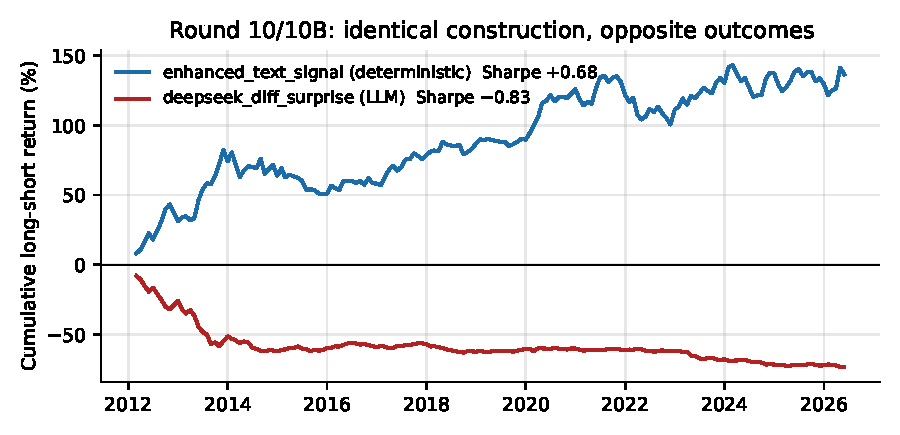
\includegraphics[width=0.86\textwidth]{fig-r10b-cumulative.pdf}
\caption{Round 10/10B cumulative long--short returns. The two signals pass through the
same parser, the same point-in-time alignment, the same sector-neutral rank-weighted
construction, and the same factor model.}
\end{figure}

\textbf{Reading.} This is the decisive result of the study, and it cuts in two directions
at once.

The LLM signal is not merely uninformative; it is \emph{anti-predictive}. Negative rank IC,
significantly negative factor alpha, and a 0th percentile against 500 random
baselines---it is worse than every random signal tested. Simultaneously, the deterministic
dictionary signal, which had looked unstable and even negative at 42 names, emerges as
genuinely positive. \textbf{One change---sample size---revealed two truths that the small
sample had been hiding at once.}

The Round 7 LLM advantage ($+0.57$ Sharpe, alpha $p = 0.045$) is therefore an artifact of
small sample plus post-hoc construction selection. This is the point at which the answer
stopped changing as the test got stricter.

\textbf{Mechanism.} The output distribution identifies the cause
(Figure~\ref{fig:dist}). Of 1,307 calls, 638 produced a non-zero score and \textbf{75.7\%
of those were negative}. More tellingly, the distribution is \emph{asymmetric in range}:
the model used the full negative half of its permitted scale down to $-5$, but never
exceeded $+3$ on the positive side. It equated ``this firm disclosed bad news'' with
``this firm will underperform''---a correct reading with an incorrect causal direction,
since disclosure is often already priced and resolution of uncertainty can itself be
favourable. Critically, this is invisible in any single output: every individual response
was well-reasoned and defensible. It appears only in aggregate.

\begin{figure}[H]
\centering
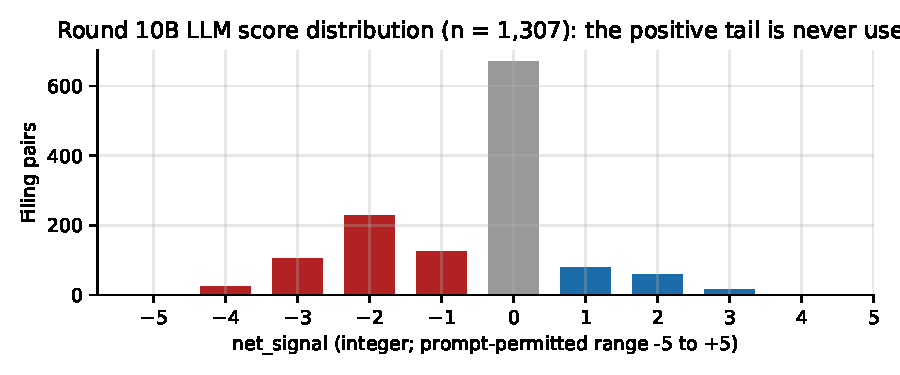
\includegraphics[width=0.86\textwidth]{fig-llm-distribution.pdf}
\caption{Round 10B score distribution. The prompt permitted $-5$ to $+5$; the model used
the entire negative range and never the top of the positive range.}
\label{fig:dist}
\end{figure}

\textbf{Infrastructure note.} During this extraction a long-running job was terminated
mid-write, truncating the output file and losing roughly 700 already-paid extractions
irrecoverably. The checkpoint had been rewriting the entire file, including a full-text
column, on every row---so the write itself was the failure point. Checkpointing was moved
to atomic write (temporary file plus rename) and the full-text column dropped, shrinking
the file roughly a hundredfold. All 1,307 extractions were re-run.

\textbf{Threat exposed $\rightarrow$ next step.} The conclusion is specific to Item 1A. The
literature suggests the productive sources are timelier ones---and within the same 10-K,
MD\&A has positive precedent.

\subsection{Round 11 --- Changing the text source, and a coverage defect}
\label{sec:r11}

\textbf{Objective.} Test whether the source, rather than the method, is the binding
constraint, using the lowest-cost available source change: MD\&A from the same filings.
No API calls; deterministic signals only. Two hypotheses were \textbf{fixed before
results were computed}:

\begin{itemize}[leftmargin=1.4em,itemsep=0.15em]
  \item \textbf{H1} \sig{mdna\_similarity}: the Lazy-Prices direction---high year-over-year
        similarity goes long.
  \item \textbf{H2} \sig{mdna\_enhanced}: the lexicon signal applied to MD\&A.
\end{itemize}

\textbf{A coverage defect found while preparing this round.} The earlier downloader read
only the \sig{recent} array of the SEC submissions API, which holds roughly the last 1,000
filings of \emph{all} types per company. For large filers this silently dropped early 10-Ks.
The Round 10 ``2012--2026'' universe was therefore not uniformly deep: the cross-section
contained as few as four names in 2012 and did not reach 100 until after 2019
(Figure~\ref{fig:cov}). Re-downloading with \sig{include\_older=True} yielded
121--150 tickers per year for 2011--2026 and raised the corpus from 1,322 to 2,146 10-Ks.
A related trap: the SEC ticker map now resolves XOM to a 2026 holding company with no 10-K
history, so Round 11 keys on CIK from the universe file instead of ticker.

\begin{figure}[H]
\centering
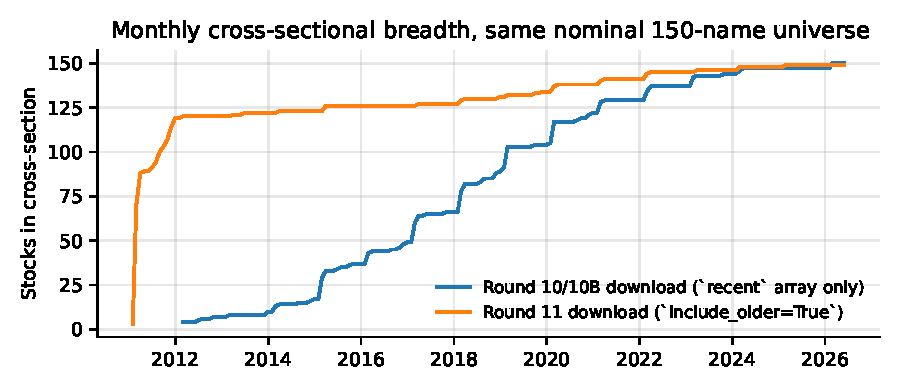
\includegraphics[width=0.86\textwidth]{fig-coverage.pdf}
\caption{Monthly cross-sectional breadth under the two download methods, for the same
nominal 150-name universe. The Round 10/10B sample was a ramp, not a panel.}
\label{fig:cov}
\end{figure}

\begin{table}[H]
\centering\small
\caption{Round 11: MD\&A and Item 1A signals on the full-coverage universe,
sector-neutral rank-weighted.}
\label{tab:r11}
\setlength{\tabcolsep}{4.5pt}\footnotesize
\begin{tabular}{l l r r r p{3.1cm}}
\toprule
\textbf{Signal} & \textbf{Role} & \textbf{Sharpe} & \textbf{vs-rand.} & \textbf{FF3+MOM alpha} & \textbf{Verdict} \\
\midrule
\sig{mdna\_similarity}   & H1          & $-0.72$ & 0.4  & $-3.6\%$, $t=-2.95$ & Significant, \textbf{sign reversed} \\
\sig{mdna\_enhanced}     & H2          & $+0.20$ & 76.8 & $+0.3\%$, $t=0.14$  & Fail \\
\sig{item1a\_enhanced}   & exploratory & $+0.49$ & 95.4 & $+2.4\%$, $t=1.88$  & Survives, weaker than Round 10 \\
\sig{item1a\_similarity} & exploratory & $+0.25$ & 81.2 & $+0.3\%$, $t=0.29$  & 2019--2026 only \\
\sig{mdna\_tone\_change} & exploratory & $+0.00$ & 52.4 & $\approx 0$         & Fail \\
\bottomrule
\end{tabular}
\end{table}

\begin{figure}[H]
\centering
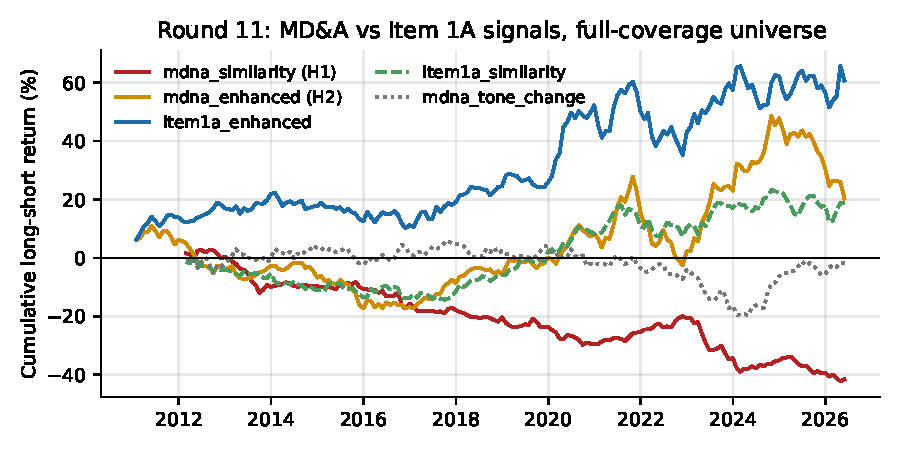
\includegraphics[width=0.86\textwidth]{fig-r11-cumulative.pdf}
\caption{Round 11 cumulative long--short returns across the five signals.}
\end{figure}

\textbf{Reading.}

\emph{H2 fails outright.} A dictionary on MD\&A produces 0.20 Sharpe and essentially zero
alpha. MD\&A tone change likewise produces nothing. The deterministic case for MD\&A as a
source is not made.

\emph{H1 is significant with the wrong sign.} High-similarity firms \emph{under}perform,
the opposite of Lazy Prices, at $-0.72$ Sharpe and alpha $t = -2.95$. The sign is robust
within sample: restricting to pairs extracted by the same method in both years gives
$-2.83$; restricting to the Item 7 layout gives $-2.70$; residualising similarity on
absolute log length change gives $-2.19$; both sub-periods are negative. The most
plausible explanation is nonetheless \textbf{survivorship bias}: in a universe of
\emph{current} index members, firms whose MD\&A changed substantially (acquisitions, new
segments, rapid growth) and which remain in the index today are survivors by construction.
``Changers outperform'' may be an artifact of who is in the sample. Since the sign was also
not the pre-registered direction, this is a post-hoc finding pending an out-of-sample test
on a point-in-time universe.

\emph{The Item 1A benchmark weakens but survives.} On full coverage it falls from 0.68 to
0.49 Sharpe, remaining at the 95th percentile versus random with FF5+MOM alpha $t = 2.12$.
The earlier, higher figure was partly a product of the thin early cross-section.

\textbf{A measurement caveat discovered in this round, applying retroactively.} The
random rank-IC percentile statistic is optimistic. Random signals are
sector/size-neutralised before their IC is computed, whereas the target signal is not, so
the random IC spread (sd $\approx 0.006$) is roughly half the target's own time-series
standard error ($\approx 0.013$). IC percentiles therefore overstate significance. Sharpe
percentiles are unaffected, because the portfolio is sector-neutral on both sides. All IC
percentiles reported in earlier rounds should be read with this in mind; Sharpe
percentiles and $t$-statistics are the reliable statistics.

%=======================================================================
\section{Synthesis: Where the Project Currently Stands}
\label{sec:synthesis}

\subsection{The trajectory}

Figure~\ref{fig:traj} plots the headline Sharpe of the best LLM signal and the
deterministic benchmark by round. The universe and construction change between rounds, so
the levels are not strictly comparable---but that is the point. The movement tracks
changes in \emph{measurement}, not changes in the underlying phenomenon.

\begin{figure}[H]
\centering
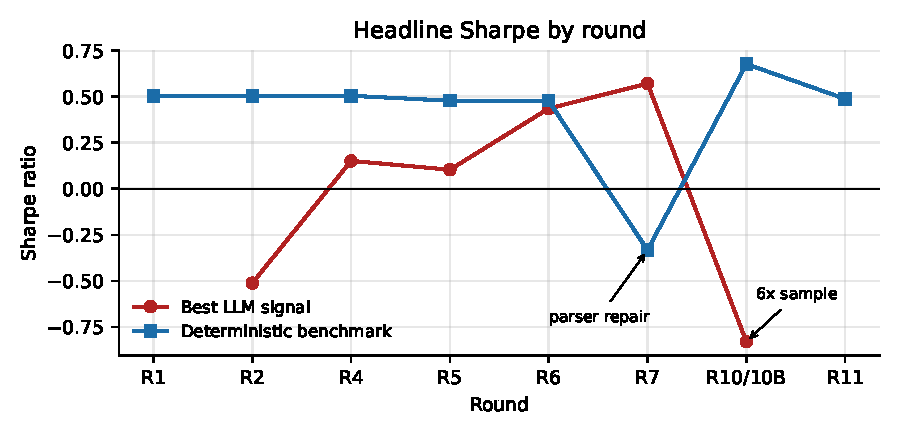
\includegraphics[width=0.86\textwidth]{fig-sharpe-by-round.pdf}
\caption{Headline Sharpe by round. Universe size and portfolio construction change between
rounds; the two largest moves coincide with the parser repair (Round 7) and the sixfold
sample expansion (Round 10B).}
\label{fig:traj}
\end{figure}

\subsection{Validity threats closed}

\begin{table}[H]
\centering\small
\caption{Each round's validity threat, the method used, and the effect on the conclusion.}
\setlength{\tabcolsep}{4pt}\footnotesize
\begin{tabular}{l p{4.3cm} p{3.6cm} p{3.9cm}}
\toprule
\textbf{Round} & \textbf{Threat} & \textbf{Method} & \textbf{Effect} \\
\midrule
1  & No control for luck & Random no-text baseline & Results gain a reference distribution \\
2  & Word counts lack semantics & LLM absolute scoring & Identifies a task-framing defect \\
3--4 & Incomplete sample & Complete the universe & $0.48 \rightarrow 0.15$ Sharpe \\
5  & Biased measurement instrument & Tie handling, persistent baseline, neutralisation & All prior rounds recomputed \\
6A & Prompt anchoring & 30-record pilot gate & Full run avoided; task identified as the issue \\
6B & Task shape & Diff + investable surprise & Healthy distribution, zero gate violations \\
6 rev.\ & Code overrode model abstention & Enforce gate in code & $0.33 \rightarrow 0.43$ Sharpe \\
7  & 42\% of inputs were wrong text & Parser repair, full re-run & Round 6 results voided \\
7b & Construction absorbing the signal & Four-way variant test & $0.07 \rightarrow 0.57$ at constant IC \\
8  & Factor exposure read as alpha & FF3/FF5+MOM, Newey--West & 91st pct.\ $\rightarrow$ marginal alpha \\
9  & Unknown scalability & Zero-API dry run & Spend de-risked \\
10/10B & Insufficient power & $6\times$ sample & Two hidden truths revealed \\
11 & Source-specific conclusion; coverage defect & MD\&A + \sig{include\_older} & 1,322 $\rightarrow$ 2,146 filings \\
\bottomrule
\end{tabular}
\end{table}

\subsection{What holds and what does not}

\textbf{Falsified.} The LLM diff-surprise approach on Item 1A, as designed. At full power
it is significantly negative, worse than every random baseline, and beaten by a word-count
dictionary on identical data. The mechanism---structural negativity bias arising from
per-item absolute scoring---is identified and is not a wording problem.

\textbf{Not supported.} MD\&A as a deterministic source. Neither the lexicon nor tone
change produces a signal, so the bar for an LLM step on MD\&A is correspondingly high.

\textbf{Holds, weakly.} The Item 1A lexicon signal: 0.49 Sharpe on full coverage, 95th
percentile versus random, FF5+MOM alpha $t = 2.12$. It carries positive market beta, so
part of the return is exposure rather than alpha, and it is only marginally significant.

\textbf{Unresolved and interesting.} The reversed MD\&A similarity effect, which is
statistically strong and robust to several within-sample checks but is confounded with
survivorship by construction.

\subsection{Transferable findings}

\begin{enumerate}[leftmargin=1.6em,itemsep=0.25em]
  \item \textbf{Most LLM failures here were context or plumbing failures, not prompt
        failures.} The parser defect, the coverage defect, and the code-override defect
        together account for more swings in the headline number than every prompt revision
        combined.
  \item \textbf{A model cannot report that its input was bad.} Independent, per-record
        input-quality instrumentation is not optional.
  \item \textbf{With no ground truth, the output distribution is the quality check.} The
        negativity bias was invisible per-response and obvious in aggregate.
  \item \textbf{A rule in a prompt is a request; a rule in code is a control.} The model
        complied perfectly with a constraint the surrounding code then violated.
  \item \textbf{Evaluate the model output and the consumption layer separately.} An
        eightfold Sharpe swing at constant rank IC is a property of the weighting scheme,
        not the model.
  \item \textbf{Statistical power is a validity threat, not a nice-to-have.} The same
        expansion that falsified the LLM signal validated the benchmark.
\end{enumerate}

%=======================================================================
\section{Limitations and Future Work}
\label{sec:limits}

\subsection{Limitations}

\begin{enumerate}[leftmargin=1.6em,itemsep=0.25em]
  \item \textbf{Survivorship and selection bias.} The universe is the alphabetically-first
        150 \emph{current} S\&P 500 members. This is the most serious threat to
        \emph{interpreting any positive result}, and it bears directly on the Round 11 H1
        finding. Because the bias inflates rather than suppresses apparent performance,
        the negative results reported here are not weakened by it.
  \item \textbf{Metadata is not point-in-time.} Sector and market-capitalisation data are
        current; price history is for currently-listed tickers.
  \item \textbf{Post-hoc construction choice.} Sector-neutral rank weighting was adopted
        after observing Round 7 variant results, weakening significance claims attached to
        it.
  \item \textbf{Gross results only.} No transaction costs, shorting costs, or capacity
        constraints.
  \item \textbf{IC percentiles overstate significance} for the reason given in
        Section~\ref{sec:r11}; Sharpe percentiles and $t$-statistics should be preferred.
  \item \textbf{Single model family.} All LLM results use one provider. Whether the
        negativity bias generalises across model families is untested.
  \item \textbf{Retroactive re-runs.} Rounds 1--10B have not been re-run on the
        full-coverage Round 11 corpus, so their levels are not directly comparable to
        Round 11's.
\end{enumerate}

\subsection{Future work, in priority order}

The ordering below follows the staging discipline that Round 9--10 established: run the
cheap, high-information experiment first, and spend on rigour once there is something
worth making rigorous.

\begin{enumerate}[leftmargin=1.6em,itemsep=0.3em]

  \item \textbf{Change the text source.} This is first because both narrative sources
        available inside the 10-K have now been tested and neither carries a usable
        signal: the LLM on Item 1A is significantly negative at full power, and on MD\&A
        neither the lexicon nor tone change produces anything. The recent literature
        concentrates almost entirely on \emph{timelier} sources---earnings-call
        transcripts, news, and standardised financial statements---and this study has
        never tested an LLM against one of them. Everything else on this list optimises
        \emph{within} a source family that has so far shown no signal.

        A new source also screens cheaply on the existing universe, and the asymmetry of
        survivorship bias makes that screen informative rather than merely convenient.
        Survivorship inflates apparent performance, so a \emph{null} on the current
        universe is strong evidence of no effect, while a \emph{positive} must be held
        back until item~2 is done. The screen is therefore safe in the direction that
        matters.

        Within this item, two design choices follow directly from the failures documented
        above, and should be adopted rather than re-derived:
        \begin{itemize}[leftmargin=1.3em,itemsep=0.1em,topsep=0.25em]
          \item \textbf{Listwise, not per-item.} Per-item absolute or incremental scoring
                is structurally prone to the negativity bias of Section~\ref{sec:results}.
                Asking the model to \emph{order} firms within a sector-year cannot inherit
                a uniform negative tilt by construction.
          \item \textbf{Extractor, not judge.} Where feasible, use embeddings with a
                controlled statistical layer (the Chen--Kelly--Xiu pattern) rather than
                having the model emit a score. This is far easier to regularise, to
                validate, and to govern.
        \end{itemize}

  \item \textbf{Point-in-time universe, including delisted firms.} This is the gate that
        must be passed before \emph{any} positive result is believed---including the
        Round 11 H1 reversal, which is statistically strong but confounded with
        survivorship by construction. It is second rather than first only because there
        is currently no live positive result that depends on it: resolving H1 alone would
        mean spending the project's next large effort confirming a post-hoc finding that
        the analysis already attributes to bias. It becomes first the moment item~1
        produces something positive, or the moment the H1 effect is to be claimed rather
        than noted.

  \item \textbf{Repair the IC baseline.} Apply identical neutralisation to the target
        signal before computing IC percentiles, and recompute the affected statistics.
        This is cheap and independent of everything else, so it can be done at any point.

  \item \textbf{Beta-neutral construction of the surviving signal.} Build a strict dollar-
        and beta-neutral version of the Item 1A lexicon signal to isolate how much
        factor-independent alpha remains once market exposure is removed. This is the
        most defensible publishable claim available from the current data.

  \item \textbf{Re-run earlier rounds on the full-coverage corpus.} Rounds 1--10B were
        computed before the filing-coverage defect of Section~\ref{sec:r11} was found, so
        their levels are not directly comparable to Round 11's. This is bookkeeping rather
        than discovery, but it is required before the cross-round trajectory is presented
        as evidence of anything.

\end{enumerate}

\subsection{What is explicitly not worth doing}

Further prompt iteration on Item 1A diff-surprise. The failure mechanism is structural,
six alternative explanations have been closed, and the result is significantly negative at
full power. Additional spend on that path would buy precision about a conclusion that is
already established.

%=======================================================================
\begin{thebibliography}{99}
\setlength{\itemsep}{0.25em}

\bibitem{campbell2014} Campbell, J.~L., Chen, H., Dhaliwal, D.~S., Lu, H., and Steele, L.~B. (2014).
The information content of mandatory risk factor disclosures in corporate filings.
\textit{Review of Accounting Studies}, 19(1), 396--455.

\bibitem{carhart1997} Carhart, M.~M. (1997). On persistence in mutual fund performance.
\textit{Journal of Finance}, 52(1), 57--82.

\bibitem{chen2024} Chen, Y., Kelly, B., and Xiu, D. (2023/24).
Expected returns and large language models. Working paper.

\bibitem{chiu2025} Chiu, C., and Hung, M. (2025).
Finance-specific large language models with LLaMA 2.
\textit{Pacific-Basin Finance Journal}, 90.

\bibitem{cohen2020} Cohen, L., Malloy, C., and Nguyen, Q. (2020). Lazy prices.
\textit{Journal of Finance}, 75(3), 1371--1415.

\bibitem{ff1993} Fama, E.~F., and French, K.~R. (1993). Common risk factors in the returns
on stocks and bonds. \textit{Journal of Financial Economics}, 33(1), 3--56.

\bibitem{ff2015} Fama, E.~F., and French, K.~R. (2015). A five-factor asset pricing model.
\textit{Journal of Financial Economics}, 116(1), 1--22.

\bibitem{huang2023} Huang, A.~H., Wang, H., and Yang, Y. (2023). FinBERT: A large language
model for extracting information from financial text.
\textit{Contemporary Accounting Research}, 40(2), 806--841.

\bibitem{kim2023} Kim, A., Muhn, M., and Nikolaev, V. (2023).
Bloated disclosures: Can ChatGPT help investors process information? Working paper.

\bibitem{kim2024} Kim, A., Muhn, M., and Nikolaev, V. (2024).
Financial statement analysis with large language models. Working paper.

\bibitem{kravet2013} Kravet, T., and Muslu, V. (2013). Textual risk disclosures and
investors' risk perceptions. \textit{Review of Accounting Studies}, 18, 1088--1122.

\bibitem{lopez2023} Lopez-Lira, A., and Tang, Y. (2023/24).
Can ChatGPT forecast stock price movements? Working paper.

\bibitem{lm2011} Loughran, T., and McDonald, B. (2011). When is a liability not a
liability? Textual analysis, dictionaries, and 10-Ks.
\textit{Journal of Finance}, 66(1), 35--65.

\bibitem{nw1987} Newey, W.~K., and West, K.~D. (1987). A simple, positive semi-definite,
heteroskedasticity and autocorrelation consistent covariance matrix.
\textit{Econometrica}, 55(3), 703--708.

\bibitem{tetlock2007} Tetlock, P.~C. (2007). Giving content to investor sentiment: The role
of media in the stock market. \textit{Journal of Finance}, 62(3), 1139--1168.

\end{thebibliography}

%=======================================================================
\appendix
\section{Reproduction}

All results are regenerated from the repository without manual steps.

\begin{table}[H]
\centering\small
\caption{Entry points by round.}
\begin{tabular}{l l}
\toprule
\textbf{Round} & \textbf{Command} \\
\midrule
7      & \sig{python3 scripts/run\_round7\_item1a\_repair\_comparison.py} \\
7b     & \sig{python3 scripts/analyze\_round7\_error\_and\_portfolio\_variants.py} \\
8      & \sig{python3 scripts/run\_round8\_factor\_regression.py} \\
9      & \sig{python3 scripts/run\_round9\_universe\_dry\_run.py} \\
9B     & \sig{python3 scripts/run\_round9b\_llm\_pilot.py} \\
10     & \sig{python3 scripts/run\_round10\_deep\_backtest.py} \\
10B    & \sig{python3 scripts/run\_round10b\_llm\_backtest.py} \\
11     & \sig{python3 scripts/download\_round11\_mdna.py} then \sig{run\_round11\_mdna\_backtest.py} \\
Figures& \sig{python3 report/make\_figures.py} \\
\bottomrule
\end{tabular}
\end{table}

Rounds 10 and 11 require no API credentials; Round 10B re-runs 1,307 paid LLM extractions.

\end{document}
